\section{Einführung}
\label{sec:Introduction}


\subsection{Grundideen}
\label{subsec:basic-concepts}
\begin{frame}
    \frametitle{\insertsubsection}
    \begin{itemize}[<+->]
        \item Was ist eine \ac{ode}?
        \item Gewöhnliche Differentialgleichungen (engl. \acp{ode}) kommen in fast allen Bereichen der Wissenschaften/Natur vor
        \item Beschreibt Änderung einer Variable
        \item ... welche von sich selbst oder anderen Variablen abhängt
    \end{itemize}
\end{frame}


\subsection{Beispiele}
\label{subsec:examples}
\begin{frame}
    \frametitle{\insertsubsection}
    \begin{itemize}[<+->]
        \item Corona-Neu-Infizierungungen (Änderung) sind proportional zu der Anzahl der bereits infizierten Menschen
        \[\dot{N} = a N\]
        \item[$\Rightarrow$] Exponentielles Wachstum $N=N_0\exp(at)$
        \item Radioaktiver Zerfall: Menge des zerfallenden Materials (Änderung) ist proportional zur Gesamtmenge
        \[\dot{N} = -\lambda N\]
        \item[$\Rightarrow$] Exponentieller Zerfall: $N=N_0\exp(-\lambda t)$
    \end{itemize}
\end{frame}


\subsection{Numerische Lösungsverfahren - Euler}
\label{subsec:numerical-methods}
\begin{frame}
    \frametitle{\insertsubsection}
    Gegeben sei eine Differentialgleichung
    \[\dot{A} = f(A, t) \hspace{1cm} A(0) = A_0\]
    Idee: berechne mit Differenzenquotienten neue Werte
    \[\lim\limits_{h\rightarrow0}\frac{A(t + h) - A(t)}{h} = f(A(t), t)\]
    Teile Zeitinterval auf in $n$ Zeitschritte $dt$.
    \[\frac{A((n+1)\cdot dt) - A(n\cdot dt)}{dt} = f(A(n\cdot dt), t)\]
    Umstellen nach $A((n+1)\cdot dt)=:A_{n+1}$ (Kurzschreibweise)
    \[A_{n+1} = A_n + dt\cdot f(A_n, n\cdot dt)\]
\end{frame}


\begin{frame}
    \frametitle{\insertsubsection}
    Zusammenfassung Verfahren: Explizites Euler-Verfahren für Gewöhnliche Differentialgleichungen:
    \begin{itemize}
        \item Solange $n\cdot dt < t_{max}$, berechne:
        \[A_{n+1} = A_n + dt\cdot f(A_n, n\cdot dt)\]
        \item Gesamtergebnis sind einzelne Werte der Funktion $A$ in dem Zeitinterval $I=[t_0, t_{max}]$
        \[I = [0, dt, 2dt, \dots, N\cdot dt]\]
        \[A = [A_0, A_1, A_2, \dots, A_N]\]
    \end{itemize}
\end{frame}


\subsection{Lösungen für \acsp{ode}}
\label{subsec:solving}
\begin{frame}[fragile]
    \frametitle{\insertsubsection}
    \begin{minted}[linenos, fontsize=\scriptsize, escapeinside=||]{python}
|\pause|import numpy as np
import matplotlib.pyplot as plt

|\pause|def A(y, t):
    return -0.5*y

|\pause|if __name__ == "__main__":
    t0 = 0.0
    tend = 10.0
    dt = 1.0
    y0 = 4.0

|\pause|    t_vals = np.arange(t0, tend, dt)
    y_vals = np.array([y0]*len(t_vals))

|\pause|    # Hier wird das Eulersche Verfahren zum lösen der ODE verwendet
    for i in range(len(y_vals)-1):
        y_vals[i+1] = y_vals[i] + dt * RHS(t_vals[i], y_vals[i])

|\pause|    plt.plot(t_vals, y_vals, label="Lösung der Differentialgleichung", marker="o")
    plt.legend()
    plt.show()
	\end{minted}
\end{frame}


\begin{frame}[fragile]
    \frametitle{\insertsubsection}
    \begin{itemize}
        \item Euler-Verfahren hat schwierigkeiten bei bestimmten "steifen" Problemen
        \item Deutlich robustere Lösungsmethoden wurden über die letzten Jahrhunderte entwickelt
        \item Wir brauchen nicht alle Details dazu kennen
        \item Gibt schon fertig entwickelte libraries, die uns die Arbeit übernehmen zB.
        \item[] \begin{minted}[fontsize=\scriptsize, escapeinside=||]{python}
from scipy.integrate import odeint
                \end{minted}
    \end{itemize}
\end{frame}


\begin{frame}[fragile]
    \frametitle{\insertsubsection}
    \begin{minted}[linenos, fontsize=\scriptsize, escapeinside=||]{python}
|\pause|import numpy as np
import matplotlib.pyplot as plt
from scipy.integrate import odeint

|\pause|def RHS(y, t):
    return -0.5*y

|\pause|if __name__ == "__main__":
    t0 = 0.0
    tend = 10.0
    dt = 1.0
    y0 = 4.0

|\pause|    t_vals = np.arange(t0, tend, dt)
|\pause|    # Hier wird eine routine von scipy zum lösen der ODE verwendet
    y_vals = odeint(RHS, y0, t_vals)

|\pause|    plt.plot(t_vals, y_vals, label="Lösung der Differentialgleichung", marker="o")
    plt.legend()
    plt.show()
	\end{minted}
\end{frame}


\begin{frame}
    \frametitle{\insertsubsection}
    \begin{figure}
        \centering
        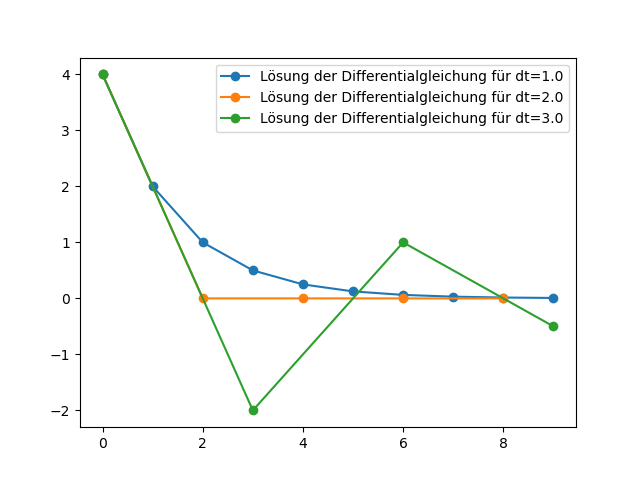
\includegraphics[width=0.7\textwidth]{media/Euler-Solutions_multiple.png}
        \caption{Das Euler-Verfahren löst eine \ac{ode} schrittweise mit konstanter Schrittweite.}
    \end{figure}
\end{frame}


\section{Aufgaben}
\subsection{Aufgabe 1}
\label{subsec:exercise-1}
\begin{frame}
    \frametitle{\insertsubsection}
    \begin{itemize}[<+->]
        \item Löse die folgende \ac{ode} mit $A(0)=2$ per Hand
        \[\dot{A} = \alpha\]
        \item Löse die folgende \ac{ode} mit $A(0)=N$ per Hand
        \[\dot{A} = - \beta A\]
        \item Welche Verhaltensweisen zeigen die Lösungen?
        \item Wie verändert sich die Lösung für verschiedene Parameter $\alpha, \beta$?
        \item Welches Biologische System könnten diese \acp{ode} beschreiben?
    \end{itemize}
\end{frame}


\subsection{Aufgabe 2}
\label{subsec:exercise-1}
\begin{frame}
    \frametitle{\insertsubsection}
    Gegeben ist die folgende Differentialgleichung
    \[\dot{A} = \alpha - \beta A\]
    mit $A(0)=0$.
    \begin{enumerate}[<+->]
        \item Löse diese Differentialgleichung numerisch mit dem Euler-Verfahren.
        \item Welche Eigenschaften haben die parameter $\alpha,\beta$?
        \item Welche Probleme können auftreten für verschiedene parameter $\alpha,\beta$?
        \item Welches biologische System könnte dieser Differentialgleichung zugrunde liegen?
    \end{enumerate}

\end{frame}


\subsection{Aufgabe 3}
\label{subsec:exercise-1}
\begin{frame}
    \frametitle{\insertsubsection}
    Wir betrachten wie eben die Differentialgleichung
    \[\dot{A} = \alpha - \beta A\]
    diesmal mit zeitabhängigem Parameter $\alpha$
    \[\alpha(t) = \left\{\begin{array}{ll}
        \alpha & 2n < t \leq 2n+1 \\
        0 & \, \textrm{sonst} \\
        \end{array}\right.\]
    \begin{itemize}[<+->]
        \item Wie können wir die Lösung dieser Differentialgleichung berechnen?
    \end{itemize}
\end{frame}


\section{Vorlesung Studienleistung}
\subsection{Projekt (Studienleistung)}
\label{subsec:project}
\begin{frame}
    \frametitle{\insertsubsection}
    \begin{itemize}[<+->]
        \item Arbeit in Gruppen (2-3 Gruppen)
        \item Erarbeiten von Model zu biologischem System
        \item Übersetzen in Computer-Simulation
        \item Diskussion der Ergebnisse in Vortrag
        \item Themen werden noch bekannt gegeben
    \end{itemize}
\end{frame}

